\documentclass[compress]{beamer}
\mode<presentation>
\usetheme{Warsaw}
\usecolortheme{seagull}

%\useoutertheme[subsection=false]{smoothbars}

%\usepackage{stackengine}
%\setbeamertemplate{caption}{\raggedright\insertcaption\par}
\setbeamertemplate{caption}{\insertcaption} 
%\usepackage{caption}
%\usepackage{pgffor}

\usepackage{fancybox}
\usepackage{minibox}
\usepackage{framed}

%\usepackage{tcolorbox}
\usepackage{empheq}


%% ====================================== graphics

\usepackage{pgfplots}
\pgfplotsset{width=10cm,compat=1.9}
%\usepgfplotslibrary{external}
%\tikzexternalize
 \usepackage{pgfplotstable}

%\definecolor{markercolor}{RGB}{.49, 1, .63}
\definecolor{markercolor}{RGB}{124.9, 255, 160.65}

\pgfplotsset{
tick label style={font=\scriptsize},
label style={font=\scriptsize},
legend style={font=\scriptsize},
title style={font=\footnotesize}
}

%% ===========================================
\usepackage{stmaryrd}

\usepackage{amsmath,amsfonts,amsthm}

% for FD grid tikz
\usepackage{tikz,amssymb}
\usetikzlibrary{calc}
\newcommand\bound{10}

\usepackage{slopetri}

\useoutertheme{infolines}
\useinnertheme{rectangles}
\usepackage{hhline}
\setbeamercovered{dynamic}

\usepackage{soul}

\usepackage{array}
\usepackage{mathrsfs}
\usepackage[utf8]{inputenc}
\usepackage{listings}
\usepackage{mathtools}
\usepackage{bm}
\usepackage{cancel}


\usepackage{graphicx}
\usepackage{subfig}
\makeatletter
\let\@@magyar@captionfix\relax
\makeatother

\usepackage{color}

\usepackage{bibentry}
\nobibliography*

\theoremstyle{plain}

% vertical bars
\newcommand*{\vertbar}{\rule[-1ex]{0.5pt}{2.5ex}}

\renewcommand{\hat}{\widehat}
\renewcommand{\tilde}{\widetilde}

%% d in integrand
\newcommand*\diff[1]{\mathop{}\!{\mathrm{d}#1}}
\newcommand{\diag}[1]{{\rm diag}\LRp{#1}}
\newcommand{\td}[2]{\frac{{\rm d}#1}{{\rm d}{\rm #2}}}
\newcommand{\pd}[2]{\frac{\partial#1}{\partial#2}}
\newcommand{\nor}[1]{\left\| #1 \right\|}
\newcommand{\LRp}[1]{\left( #1 \right)}
\newcommand{\LRs}[1]{\left[ #1 \right]}
\newcommand{\LRa}[1]{\left\langle #1 \right\rangle}
\newcommand{\LRb}[1]{\left| #1 \right|}
\newcommand{\LRc}[1]{\left\{ #1 \right\}}
\newcommand{\LRceil}[1]{\left\lceil #1 \right\rceil}
\newcommand{\LRu}[1]{\left. #1 \right|}
\newcommand{\pdn}[3]{\frac{\partial^{#3}#1}{\partial#2^{#3}}}
\newcommand{\Grad} {\ensuremath{\nabla}}
\newcommand{\jump}[1] {\ensuremath{\llbracket#1\rrbracket}}
\newcommand{\avg}[1] {\ensuremath{\LRc{\!\{#1\}\!}}}

\graphicspath{{./figs/}}

\renewcommand{\note}[1]{\textcolor{red}{{#1}}}
%\renewcommand{\note}[1]{{\color{blue}{#1}}}


% removes nav symbols
\beamertemplatenavigationsymbolsempty
%\setbeamertemplate{caption}{\raggedright\insertcaption\par}

% defines newblock as null, giving compile issues otherwise
\let\newblock\relax 


\title[Entropy stable DG for SWE]{A discretely entropy stable discontinuous Galerkin method for the shallow water equations}
\date[7/31/19]{USNCCM 15, Austin, TX\\July 31, 2019}
\author[J.\ Chan, P.\ Wu]{Jesse Chan, Philip Wu}
\institute[Rice CAAM]{\inst{1}Department of Computational and Applied Mathematics}

\begin{document}
\makeatletter
\@addtoreset{subfigure}{framenumber}% subfigure counter resets every frame
\makeatother

\begin{frame}
\maketitle
\end{frame}

%% =================================================

\frame{
\frametitle{Why high order discontinuous Galerkin methods?}

\vspace{-.5em}
\begin{columns}
\begin{column}{.65\textwidth}
Discontinuous Galerkin (DG) methods: 
\vspace{.5em}
\begin{itemize}
\item Geometric flexibility, high order accuracy.
\vspace{.5em}
\item Weak continuity across faces.
\end{itemize}
\end{column}
\begin{column}{.35\textwidth}
\vspace{-.5em}
\begin{figure}
\centering
\includegraphics[width=\textwidth]{figs/dg.pdf}
\end{figure}
\end{column}
\end{columns}

\vspace{.5em}
\begin{itemize}
\item Continuous PDE (example: advection)
\[
\pd{u}{t}{} = \pd{f(u)}{x}{}, \qquad f(u) = u.
\]
\item Local DG form with numerical flux $\bm{f}^*$: find $u \in P^N\LRp{D^k}$ such that
\[
\int_{D_k}\pd{u}{t} \phi = \int_{D_k}\pd{f(u)}{x}\phi + \int_{\partial D_k}{\bm{n}\cdot\LRp{\bm{f}^*-\bm{f}(u)}\phi}, \qquad \forall \phi \in P^N\LRp{D^k}.
\]
\end{itemize}
}

\frame[noframenumbering]{
\frametitle{Why high order discontinuous Galerkin methods?}

\begin{figure}
\only<1>{
\setcounter{subfigure}{0}
\centering
\vspace{-.1em}
\includegraphics[width=.35\textwidth]{figs/advec1d_N0_diss.png}
\hspace{2em}
\includegraphics[width=.35\textwidth]{figs/advec1d_N1_diss.png}\\[.5em]
\hspace{.75em}
\includegraphics[width=.35\textwidth]{figs/advec1d_N3_diss.png}
\hspace{2em}
\includegraphics[width=.35\textwidth]{figs/advec1d_N7_diss.png}
}
\only<2>{
\centering
\vspace{1em}
\includegraphics[width=.925\textwidth]{figs/turbulent1.png}\\
\vspace{.5em}
\includegraphics[width=.925\textwidth]{figs/turbulent2.png}
\caption*{\footnotesize 8th order simulation of forced Kelvin-Helmholtz instability (Per-Olof Persson).  Vorticular structures and acoustic forcing are both sensitive to numerical dissipation.}
}
\end{figure}

\begin{center}
High order accurate resolution of propagating vortices and waves.
\end{center}

%\begin{center}
%Simplified explicit time-stepping (mass matrix inversion)
%\end{center}
%\only<4->{\includegraphics[width=.65\textwidth]{figs/dg.pdf}}
%\only<4>{\includegraphics[width=.65\textwidth]{figs/MCG.pdf}\caption*{\footnotesize High order FEM mass matrix.}}
%\only<5>{\includegraphics[width=.65\textwidth]{figs/MDG.pdf}\caption*{\footnotesize High order DG mass matrix.}}
}

\frame[noframenumbering]{
\frametitle{Why high order discontinuous Galerkin methods?}

\begin{figure}
\centering
\includegraphics[width=.3\textwidth]{figs/cg.pdf}
\hspace{1em}
\includegraphics[width=.3\textwidth]{figs/dg.pdf}\\
\subfloat[High order FEM]{\includegraphics[width=.3\textwidth]{figs/MCG.pdf}}
\hspace{1em}
\subfloat[High order DG]{\includegraphics[width=.3\textwidth]{figs/MDG.pdf}}
\caption*{\footnotesize Simple high order mass matrix for explicit time-stepping on unstructured meshes.}
\end{figure}

%\begin{center}
%Simplified explicit time-stepping (mass matrix inversion)
%\end{center}
%\only<4->{\includegraphics[width=.65\textwidth]{figs/dg.pdf}}
}



\frame{
\frametitle{Why \textit{not} high order DG methods?}
\setcounter{subfigure}{0}
\vspace{-1em}
\begin{figure}
\begin{overprint}
\centering
\foreach \id in {1,2,3,4}{%
\only<\id>{
\captionsetup[subfloat]{width=.45\textwidth, justification=centering}
\subfloat[Exact solution]{%[$N = 7, K = 8$ (aligned mesh)]{
\makebox[.425\textwidth]{\includegraphics[width=.4\textwidth]{figs/burgersStable_\id.png}}}%
\hspace{1em}%
\subfloat[8th order DG]{ %[$N = 7, K = 9$ (non-aligned mesh)]{
\makebox[.425\textwidth]{\includegraphics[width=.4\textwidth]{figs/burgersUnstable_\id.png}}}
} % only
} % foreach 
\end{overprint}
\end{figure}
%\vspace{-.5em}
\begin{itemize}
\item High order methods blow up for under-resolved solutions of \note{nonlinear conservation laws} (e.g., shocks and turbulence).   
\vspace{.25em}
\item Instability tied to loss of the \note{chain rule} + \note{quadrature error}.  
\end{itemize}
}


\frame{
\frametitle{Entropy stability for nonlinear problems}
\vspace{-.5em}
\begin{itemize}
\item Generalizes energy stability to \note{nonlinear} systems of conservation laws (Burgers', shallow water, compressible Euler, MHD).  
\[
\pd{\bm{u}}{t} + \pd{\bm{f}(\bm{u})}{x} = 0.  
\]
\item Continuous entropy inequality: given a convex \note{entropy} function $S(\bm{u})$ and ``entropy potential'' $\psi(\bm{u})$, 
\begin{align*}
&\int_{\Omega} \bm{v}^T\LRp{\pd{\bm{u}}{t} + \pd{\bm{f}(\bm{u})}{x}} = 0, \qquad \boxed{\bm{v} = \pd{S}{\bm{u}}} \\
&\Longrightarrow \int_{\Omega}\pd{S(\bm{u})}{t} + \LRu{\LRp{\bm{v}^T\bm{f}(\bm{u}) - \psi(\bm{u})}}_{-1}^1 \leq 0.
\end{align*}
\vspace{.01em}
\item Proof of entropy inequality relies on \note{chain rule}, integration by parts.  
\end{itemize}
}

\frame{
\frametitle{Discretely entropy stable schemes: main ideas}

\begin{itemize}
\item<1-> Continuous and semi-discrete systems
\[
\boxed{\pd{\bm{u}}{t} + \pd{\bm{f}(\bm{u})}{x} - \epsilon \pdn{u}{x}{2}= 0} \quad \Longrightarrow \quad
\boxed{\bm{M}\td{\bm{u}}{t} + \bm{Q}\bm{f}(\bm{u}) + \epsilon \bm{K}\bm{u} = \bm{0}}
%\boxed{\td{\bm{u}}{t} + \bm{D}\bm{f}(\bm{u}) + \epsilon \bm{K}\bm{u} = \bm{0}}
\]
\item<2-> Test with discrete entropy variables, use chain rule in time
\[
\underbrace{\bm{v}^T\bm{M}\td{\bm{u}}{t}}_{\bm{1}^T\bm{M}\td{S(\bm{u})}{t}} + \bm{v}^T\bm{Q}\bm{f}(\bm{u}) + \epsilon \bm{v}^T\bm{K}\bm{u} = \bm{0}
%\boxed{\td{\bm{u}}{t} + \bm{D}\bm{f}(\bm{u}) + \epsilon \bm{K}\bm{u} = \bm{0}}
\]
\item<3-> Construct discretization s.t.\ (for periodic boundary conditions)
\[
\boxed{
\begin{array}{c}
\textcolor{red}{\bm{v}^T\bm{Q}\bm{f}(\bm{u}) = 0}\\
\bm{v}^T\bm{K}\bm{u} \geq 0
\end{array}
} \qquad \Longrightarrow \qquad \bm{1}^T\bm{M}\td{S(\bm{u})}{t} = -\epsilon \bm{v}^T\bm{K}\bm{u} \leq 0.
\]
\end{itemize}
}

\frame{
\frametitle{Illustrative example of discrete entropy stability}
\vspace{-.5em}
\begin{figure}
\begin{overlayarea}{\textwidth}{.45\textheight}
\centering
\only<1>{
\subfloat[Entropy conservative flux, $T = .3$]{\includegraphics[width=.49\textwidth]{figs/shockVortexTp3_EC.png}}
\hspace{.05em}
\subfloat[Entropy conservative flux, $T = .7$]{\includegraphics[width=.49\textwidth]{figs/shockVortexTp7_EC.png}}
}
%\only<2>{
%\subfloat[Local Lax-Friedrichs flux, $T = .3$]{\includegraphics[width=.49\textwidth]{figs/shockVortexTp3_LF.png}}
%\hspace{.05em}
%\subfloat[Local Lax-Friedrichs flux, $T = .7$]{\includegraphics[width=.49\textwidth]{figs/shockVortexTp7_LF.png}}\
%}
\only<2>{
\subfloat[Upwind-like flux, $T = .3$]{\includegraphics[width=.49\textwidth]{figs/shockVortexTp3.png}}
\hspace{.05em}
\subfloat[Upwind-like flux, $T = .7$]{\includegraphics[width=.49\textwidth]{figs/shockVortexTp7.png}}
}
\only<3>{
\subfloat[Upwind-like flux, $T = .3$]{\includegraphics[width=.485\textwidth]{figs/shockVortexT3.png}}
\hspace{.05em}
\subfloat[Upwind-like flux, $T = .7$]{\includegraphics[width=.49\textwidth]{figs/shockVortexT7.png}}
}
\end{overlayarea}
\caption{\footnotesize Compressible Euler shock vortex interaction: $200\times 100$ \note{degree $N=4$} elements, $4$th order \note{explicit} RK time-stepping, no limiters or artificial viscosity.}
\end{figure}

\begin{center}
For physically relevant solutions (e.g., positive density), high order entropy stable schemes remain stable without any additional dissipation.
\end{center}
}

\section{Summation by parts and flux differencing}

\frame[noframenumbering]{
\frametitle{Talk outline}
\tableofcontents
}
\frame[noframenumbering]{
\frametitle{Talk outline}
\tableofcontents[currentsection]
}

\frame{
\frametitle{Nodal DG, summation-by-parts, flux differencing}
\setcounter{subfigure}{0}

\begin{overlayarea}{\textwidth}{\textheight}
\vspace{-.25em}
\begin{figure}
\centering
\subfloat{\includegraphics[width=.4\textwidth]{figs/gll1Dsbp.pdf}}
\hspace{2.5em}
\subfloat{\raisebox{.475em}{\includegraphics[width=.33\textwidth]{figs/B_SBP.png}}}
\end{figure}
\only<1>{
\begin{itemize}
\item \note{Nodal} differentiation matrix $\bm{D}$ with zero row sums
\vspace{.25em}
\[
\bm{D}\bm{1} = 0 \qquad \Longrightarrow \qquad \sum_{j} \bm{D}_{ij} = 0, \quad (\bm{D} \text{ exact for constants})
\]
\item \note{Lobatto nodes} mimic {integration by parts} (summation-by-parts) % using differentiation matrix $\bm{D}$, diagonal (lumped) mass matrix $\bm{M}$, boundary matrix $\bm{B}$
\vspace{.25em}
\[
\bm{Q} = \bm{M}\bm{D}, \qquad \boxed{\bm{Q} = \bm{B} - \bm{Q}^T,} \qquad \bm{M} \text{ diagonal mass matrix}.
\]
%\vspace{.01em}
\end{itemize}
}
\only<2->{
\vspace{-.5em}
\begin{itemize}
\item<2-> {Nodal} ``collocation'' over a single element:
\[
\int\pd{\bm{f}(\bm{u})}{x} v(x) \approx \bm{Q}\bm{f}(\bm{u})  \quad  \Longrightarrow \quad \sum_{j} \bm{Q}_{ij} \bm{f}\LRp{\bm{u}_j}.
\]
\item<3> Let $\bm{f}_S(\bm{u}_i,\bm{u}_j) = \frac{1}{2}\LRp{\bm{f}(\bm{u}_i)+\bm{f}(\bm{u}_j)} = {\bm{F}}_{ij}$.  Replace $\bm{Q}\bm{f}(\bm{u})$ with
\[
\sum_{j} \bm{Q}_{ij} \note{2\bm{f}_S\LRp{\bm{u}_i,\bm{u}_j}} \quad \Longrightarrow \quad \boxed{2\LRp{\bm{Q}\circ\note{\bm{F}}}\bm{1} = 0.}
\]
\end{itemize}
}
\end{overlayarea}
}


\frame{
\frametitle{Entropy stable nodal DG: a brief summary}

\begin{itemize}
\item Trick: use Tadmor's entropy conservative numerical flux for $\bm{f}_S$
\vspace{-.25em}
\begin{align*}
\bm{f}_S(\bm{u},\bm{u}) &= \bm{f}(\bm{u}), \qquad \text{(consistency)} \\
\bm{f}_S(\bm{u},\bm{v}) &= \bm{f}_S(\bm{v},\bm{u}),\qquad \text{(symmetry)} \\
\LRp{\bm{v}_L - \bm{v}_R}^T \bm{f}_S\LRp{\bm{u}_L,\bm{u}_R} &= \psi_L - \psi_R, \qquad \text{(conservation)}.
\end{align*}
\item If \note{$\bm{Q}\bm{1} = \bm{0}$} and $\bm{Q}$ satisfies the \note{summation-by-parts} property, then the following (local) formulation is entropy conservative  
\[
\boxed{\bm{M}\td{\bm{u}}{t} + 2\LRp{\bm{Q}\circ\bm{F}}\bm{1} + \bm{B}\LRp{\bm{f}_S\LRp{\bm{u}^+,\bm{u}}-\bm{f}(\bm{u})} = \bm{0}}
\]
\item Adding Lax-Friedrichs dissipation produces an \note{entropy stable} scheme.
\[
\bm{f}_S\LRp{\bm{u}^+,\bm{u}} - \frac{\lambda}{2} \jump{\bm{u}}, \qquad \text{$\lambda$ estimates maximum wavespeed.}
\]
%\item<6-> Proof of entropy balance: multiply by $\bm{v}^T$
%\begin{overlayarea}{\textwidth}{.175\textheight}
%\[
%\hspace*{-1em}
%\only<1-6>{\bm{v}^T\bm{M}\td{\bm{u}}{t} + \bm{v}^T\LRp{\LRp{\bm{Q}-\bm{Q}^T}\circ\bm{F}_S}\bm{1} + \bm{v}^T\bm{B}\bm{f}^* = 0.}
%\only<7>{\bm{1}^T\bm{M}\td{S(\bm{u})}{t} + \sum_{ij} \bm{Q}_{ij} \note{\LRp{\bm{v}_i-\bm{v}_j}^T \bm{f}_S\LRp{\bm{u}_i,\bm{u}_j}} + \bm{v}^T\bm{B}\bm{f}^* = 0.}
%\only<8>{\bm{1}^T\bm{M}\td{S(\bm{u})}{t} + \sum_{ij} \bm{Q}_{ij} \note{\LRp{\psi(\bm{u}_i)-\psi(\bm{u}_j)}} + \bm{v}^T\bm{B}\bm{f}^* = 0.}
%\only<9>{\bm{1}^T\bm{M}\td{S(\bm{u})}{t} + \note{\bm{\psi}^T\bm{Q}\bm{1} - \bm{1}^T\bm{Q}\bm{\psi}} + \bm{v}^T\bm{B}\bm{f}^* = 0.}
%\only<10>{\bm{1}^T\bm{M}\td{S(\bm{u})}{t} + \bm{1}^T\bm{B}\LRp{\bm{v}^T\bm{f}^* - \bm{\psi}}  = 0.}
%\only<11>{\bm{1}^T\bm{M}\td{S(\bm{u})}{t} + \bm{1}^T\bm{B}\LRp{\bm{v}^T\bm{f}^* - \bm{\psi}}  \leq 0 \text{ \note{(if dissipation added)}}.}
%\]
%\end{overlayarea}
\end{itemize}
%\let\thefootnote\relax\footnotetext{\tiny Tadmor, Eitan (1987), Fisher and Carpenter (2014), Gassner, Winters, and Kopriva (2016).}
}

%\frame{
%%\frametitle{Entropy stable schemes: a brief derivation}
%\vspace{1em}
%\begin{itemize}
%%\item Define $\bm{f}_S, \bm{f}^*$ using Tadmor's entropy conservative numerical flux
%%\begin{align*}
%%%\bm{f}_S(\bm{u},\bm{u}) &= \bm{f}(\bm{u}), \qquad \text{(consistency)} \\
%%%\bm{f}_S(\bm{u},\bm{v}) &= \bm{f}_S(\bm{v},\bm{u}),\qquad \text{(symmetry)} \\
%%\LRp{\bm{v}_L - \bm{v}_R}^T \bm{f}_S\LRp{\bm{u}_L,\bm{u}_R} &= \psi_L - \psi_R, \qquad \text{(conservation)}.
%%\end{align*}
%%\vspace{.5em}
%\item Tadmor's entropy conservative condition
%\[
%\LRp{\bm{v}_L - \bm{v}_R}^T \bm{f}_S\LRp{\bm{u}_L,\bm{u}_R} = \psi_L - \psi_R, \qquad \text{(conservation)}.
%\]
%\vspace{.01em}
%\item Multiply by $\bm{v}^T$ to derive semi-discrete entropy balance: 
%\begin{overlayarea}{\textwidth}{.55\textheight}
%\[
%\bm{v}^T\bm{M}\td{\bm{u}}{t} + \bm{v}^T\LRp{\LRp{\bm{Q}-\bm{Q}^T}\circ\bm{F}_S}\bm{1} + \bm{v}^T\bm{B}\bm{f}^* = 0.
%\]
%\uncover<2->{
%\[
%\Longrightarrow \bm{1}^T\bm{M}\td{S(\bm{u})}{t} + \sum_{ij} \bm{Q}_{ij} \underbrace{\note{\LRp{\bm{v}_i-\bm{v}_j}^T \bm{f}_S\LRp{\bm{u}_i,\bm{u}_j}}}_{\text{Tadmor's condition}} + \bm{v}^T\bm{B}\bm{f}^* = 0.
%\]
%}
%\uncover<3->{
%\[
%\only<1-3>{\Longrightarrow \bm{1}^T\bm{M}\td{S(\bm{u})}{t} + \sum_{ij} \bm{Q}_{ij} \note{\LRp{\psi(\bm{u}_i)-\psi(\bm{u}_j)}} + \bm{v}^T\bm{B}\bm{f}^* = 0.}
%\only<4>{\Longrightarrow \bm{1}^T\bm{M}\td{S(\bm{u})}{t} + \note{\bm{\psi}^T\bm{Q}\bm{1} - \bm{1}^T\bm{Q}\bm{\psi}} + \bm{v}^T\bm{B}\bm{f}^* = 0.}
%\only<5>{\Longrightarrow \bm{1}^T\bm{M}\td{S(\bm{u})}{t} + \bm{1}^T\bm{B}\LRp{\bm{v}^T\bm{f}^* - \bm{\psi}}  = 0.}
%\only<6>{\Longrightarrow \bm{1}^T\bm{M}\td{S(\bm{u})}{t} + \bm{1}^T\bm{B}\LRp{\bm{v}^T\bm{f}^* - \bm{\psi}}  \leq 0, \quad \text{(added dissipation)}.}
%\]
%}
%\end{overlayarea}
%\end{itemize}
%\let\thefootnote\relax\footnotetext{\tiny Tadmor, Eitan (1987), Fisher and Carpenter (2014), Gassner, Winters, and Kopriva (2016).}
%}


%\frame{
%\frametitle{Nodal DG, summation-by-parts (SBP), flux differencing}
%\setcounter{subfigure}{0}
%
%\begin{overlayarea}{\textwidth}{\textheight}
%\vspace{-.25em}
%\begin{figure}
%\centering
%\subfloat{\includegraphics[width=.375\textwidth]{figs/gll1Dsbp.pdf}}
%\hspace{2.5em}
%\subfloat{\raisebox{.475em}{\includegraphics[width=.3\textwidth]{figs/B_SBP.png}}}
%\end{figure}
%\only<1>{
%\begin{itemize}
%\item Nodal differentiation matrix $\bm{D}$ exact for constants
%\vspace{.25em}
%\[
%\bm{D}\bm{1} = 0 \qquad \Longrightarrow \qquad \sum_{j} \bm{D}_{ij} = 0, \quad (\text{zero row sums})
%\]
%\item Lobatto quadrature nodes mimic \note{integration by parts} algebraically % using differentiation matrix $\bm{D}$, diagonal (lumped) mass matrix $\bm{M}$, boundary matrix $\bm{B}$
%\vspace{.25em}
%\[
%\boxed{\bm{Q} = \bm{B} - \bm{Q}^T,} \qquad \bm{Q} = \bm{M}\bm{D}, \qquad \bm{M} \text{ diagonal mass matrix}.
%\]
%%\vspace{.01em}
%\end{itemize}
%}
%\only<2->{
%\vspace{-.75em}
%\begin{itemize}
%\item<2-> Nodal ``collocation'' over a single element:
%\[
%\bm{M}\td{\bm{u}}{t} + \bm{Q}\bm{f}(\bm{u}) = 0 \quad  \Longrightarrow \quad \bm{M}_{ii}\td{\bm{u}_i}{t} + \sum_{j} \bm{Q}_{ij} \bm{f}\LRp{\bm{u}_j} = 0.
%\]
%\item<3> Let $\bm{f}_S(\bm{u}_i,\bm{u}_j) = \frac{1}{2}\LRp{\bm{f}(\bm{u}_i)+\bm{f}(\bm{u}_j)} = \LRp{\bm{F}_S}_{ij}$.  Collocation equiv.\ to
%\[
%\bm{M}_{ii}\td{\bm{u}_i}{t} + \sum_{j} \bm{Q}_{ij} \note{2\bm{f}_S\LRp{\bm{u}_i,\bm{u}_j}} = 0 \quad \Longrightarrow \quad \boxed{\bm{M}\td{\bm{u}}{t} + 2\LRp{\bm{Q}\circ\note{\bm{F}_S}}\bm{1} = 0.}
%\]
%\end{itemize}
%}
%\end{overlayarea}
%
%}
%
%
%
%\frame{
%\frametitle{Deriving entropy stable schemes}
%
%\begin{itemize}
%\item<1-> Derive formulation with boundary (interface) flux $\bm{f}^*$
%\begin{overlayarea}{\textwidth}{.17\textheight}
%\vspace{-1em}
%\begin{align*}
%\only<1>{\bm{M}\td{\bm{u}}{t} + 2\LRp{\bm{Q}\circ\bm{F}_S}\bm{1} = 0}
%\only<2>{\bm{M}\td{\bm{u}}{t} + \underbrace{\LRp{\LRp{\note{\bm{Q}-\bm{Q}^T}}\circ\bm{F}_S}\bm{1}}_{\text{SBP property}} + \LRp{\note{\bm{B}}\circ\bm{F}_S}\bm{1} = 0}
%\only<3>{\bm{M}\td{\bm{u}}{t} + \LRp{\LRp{\bm{Q}-\bm{Q}^T}\circ\bm{F}_S}\bm{1} + \underbrace{\note{\bm{B}\bm{f}(\bm{u})}}_{\LRp{\bm{F}_S}_{ii} = \bm{f}(\bm{u}_i) \text{ + diagonal } \bm{B}}  = 0.}
%\only<4>{\bm{M}\td{\bm{u}}{t} + \LRp{\LRp{\bm{Q}-\bm{Q}^T}\circ\bm{F}_S}\bm{1} + \underbrace{\note{\bm{B}\bm{f}^*}}_{\text{Numerical flux}} = 0.  }
%\only<5->{\bm{M}\td{\bm{u}}{t} + \LRp{\LRp{\bm{Q}-\bm{Q}^T}\circ\bm{F}_S}\bm{1} + \bm{B}\bm{f}^* = 0.  }
%\end{align*}
%\end{overlayarea}
%\item<6-> Trick: use Tadmor's entropy conservative numerical flux for $\bm{f}_S, \bm{f}^*$
%\begin{align*}
%\bm{f}_S(\bm{u},\bm{u}) &= \bm{f}(\bm{u}), \qquad \text{(consistency)} \\
%\bm{f}_S(\bm{u},\bm{v}) &= \bm{f}_S(\bm{v},\bm{u}),\qquad \text{(symmetry)} \\
%\LRp{\bm{v}_L - \bm{v}_R}^T \bm{f}_S\LRp{\bm{u}_L,\bm{u}_R} &= \psi_L - \psi_R, \qquad \text{(conservation)}.
%\end{align*}
%\item<7-> Entropy \note{conservation}: multiply by $\bm{v}(\bm{u})^T$, chain rule in time
%\begin{overlayarea}{\textwidth}{.175\textheight}
%\[
%\hspace*{-1em}
%\only<1-7>{\bm{v}^T\bm{M}\td{\bm{u}}{t} + \bm{v}^T\LRp{\LRp{\bm{Q}-\bm{Q}^T}\circ\bm{F}_S}\bm{1} + \bm{v}^T\bm{B}\bm{f}^* = 0.}
%\only<8>{\bm{1}^T\bm{M}\td{S(\bm{u})}{t} + \sum_{ij} \bm{Q}_{ij} \note{\LRp{\bm{v}_i-\bm{v}_j}^T \bm{f}_S\LRp{\bm{u}_i,\bm{u}_j}} + \bm{v}^T\bm{B}\bm{f}^* = 0.}
%\only<9>{\bm{1}^T\bm{M}\td{S(\bm{u})}{t} + \sum_{ij} \bm{Q}_{ij} \note{\LRp{\psi(\bm{u}_i)-\psi(\bm{u}_j)}} + \bm{v}^T\bm{B}\bm{f}^* = 0.}
%\only<10>{\bm{1}^T\bm{M}\td{S(\bm{u})}{t} + \note{\bm{\psi}^T\bm{Q}\bm{1} - \bm{1}^T\bm{Q}\bm{\psi}} + \bm{v}^T\bm{B}\bm{f}^* = 0.}
%\only<11>{\bm{1}^T\bm{M}\td{S(\bm{u})}{t} + \bm{1}^T\bm{B}\LRp{\bm{v}^T\bm{f}^* - \bm{\psi}}  = 0.}
%\only<12>{\bm{1}^T\bm{M}\td{S(\bm{u})}{t}  = 0, \qquad \text{(for periodic domains)}.}
%\]
%\end{overlayarea}
%\end{itemize}
%\let\thefootnote\relax\footnotetext{\tiny Tadmor, Eitan (1987), Gassner, Winters, and Kopriva (2016).}
%}
%
%\frame{
%\frametitle{Example: entropy stability for Burgers' equation }
%\setcounter{subfigure}{0}
%
%\begin{figure}
%\begin{overlayarea}{\textwidth}{.5\textheight}
%%\begin{overprint}
%\centering
%\foreach \id in {1,2,3,4,5,6,7,8}{%
%\only<\id>{
%\subfloat[Energy conservative ($\tau = 0$)]{\includegraphics[width=.425\textwidth]{figs/burgersStableEC_\id.png}}\hspace{2em}%
%\subfloat[Energy stable ($\tau = 1$)]{\includegraphics[width=.425\textwidth]{figs/burgersStableLF_\id.png}}
%}% \only
%}% for
%\only<9>{
%\captionsetup[subfloat]{width=.45\textwidth, justification=centering}
%\subfloat[Entropy over time for $\tau = 0$]{\includegraphics[width=.45\textwidth]{figs/burgersSplitEnergyEC.png}}\hspace{1em}%
%\subfloat[Entropy over time for $\tau = 1$]{\includegraphics[width=.45\textwidth]{figs/burgersSplitEnergyLF.png}}
%}
%%\end{overprint}
%\end{overlayarea}
%\vspace{1em}
%\[
%\boxed{\pd{u}{t} + \frac{1}{2}\pd{u^2}{x} = 0, \qquad S(u) = \frac{u^2}{2}.}
%\]
%\end{figure}
%}
%
%\frame{
%\frametitle{What is flux differencing doing?}
%\begin{itemize}
%\item<1-> Entropy conservative flux for Burgers' equation 
%\[
%f_S(u_L,u_R) = \frac{1}{6}\LRp{u_L^2 + u_Lu_R + u_R^2}, \qquad f_S(u,u) = f(u) = \frac{u^2}{2}.
%\]
%\item<1-> Flux differencing: let $u_L = u(x), u_R = u(y)$
%\[
%%\only<1->{\pd{{f}({u})}{x} \Longrightarrow \pd{f(u)}{u} \pd{u}{x}}
%%\only<2->{\pd{{f}({u})}{x} \Longrightarrow \pd{f_S(u,u)}{u}\pd{u}{x}}
%%\only<1->{
%\pd{{f}({u})}{x} \Longrightarrow \note{\LRu{2\pd{f_S\LRp{u(x),u(y)}}{x}}_{y=x}}
%%}
%\]
%\item<2-> Recovers a known stable split form of Burgers' equation
%\begin{gather*}
%f_S(u(x),u(y)) = \frac{1}{6}\LRp{u(x)^2 + u(x)u(y) + u(y)^2}\\
%\LRu{2\pd{f_S\LRp{u(x),u(y)}}{x}}_{y=x} = \frac{1}{3}\pd{u^2}{x} + \frac{1}{3}u\pd{u}{x} + \frac{1}{3}u^2\cancel{\pd{1}{x}}.
%\end{gather*}
%\end{itemize}
%}
%
%%\frame{
%%\frametitle{Flux differencing: beyond split formulations}
%%\begin{itemize}
%%\item Fluxes $\bm{f}_S$ do not necessarily correspond to split formulations!  
%%\vspace{.5em}
%%\item Example: entropy conservative flux for 1D compressible Euler
%%\begin{align*}
%%f^1_S(\bm{u}_L,\bm{u}_R) &= \avg{\rho}^{\log} \avg{u}\\
%%f^2_S(\bm{u}_L,\bm{u}_R) &= \frac{\avg{\rho}}{2\avg{\beta}} + \avg{u}f^1_S\\
%%f^3_S(\bm{u}_L,\bm{u}_R) &= f^1_S\LRp{\frac{1}{2(\gamma-1)\avg{\beta}^{\log}} - \frac{1}{2}\avg{u^2}} + \avg{u}f^2_S,
%%\end{align*}
%%%\vspace{.5em}
%%\item Rational functions: logarithmic mean and ``inverse temperature'' $\beta$
%%\[
%%\avg{u}^{\log} = \frac{u_L - u_R}{\log{u_L}- \log{u_R}}, \qquad \beta = \frac{\rho}{2p}.
%%\]
%%\end{itemize}
%%
%%\let\thefootnote\relax\footnotetext{\tiny Chandreshekar (2013),  \emph{Kinetic energy preserving and entropy stable FV schemes for comp.\ Euler and NS equations.}}
%%}
%%
%
%\frame{
%\frametitle{Beyond split formulations: compressible Euler}
%\vspace{-.5em}
%\begin{figure}
%\centering
%\begin{overlayarea}{\textwidth}{.4\textheight}
%\only<1>{
%\subfloat[Entropy conservative flux, $T = .3$]{\includegraphics[width=.49\textwidth]{figs/shockVortexTp3_EC.png}}
%\hspace{.05em}
%\subfloat[Entropy conservative flux, $T = .7$]{\includegraphics[width=.49\textwidth]{figs/shockVortexTp7_EC.png}}
%}
%\only<2>{
%\subfloat[Local Lax-Friedrichs flux, $T = .3$]{\includegraphics[width=.49\textwidth]{figs/shockVortexTp3_LF.png}}
%\hspace{.05em}
%\subfloat[Local Lax-Friedrichs flux, $T = .7$]{\includegraphics[width=.49\textwidth]{figs/shockVortexTp7_LF.png}}\
%}
%\only<3>{
%\subfloat[Matrix dissipation flux, $T = .3$]{\includegraphics[width=.49\textwidth]{figs/shockVortexTp3.png}}
%\hspace{.05em}
%\subfloat[Matrix dissipation flux, $T = .7$]{\includegraphics[width=.49\textwidth]{figs/shockVortexTp7.png}}
%}
%\only<4>{
%\subfloat[Matrix dissipation flux, $T = .3$]{\includegraphics[width=.485\textwidth]{figs/shockVortexT3.png}}
%\hspace{.05em}
%\subfloat[Matrix dissipation flux, $T = .7$]{\includegraphics[width=.49\textwidth]{figs/shockVortexT7.png}}
%}
%\end{overlayarea}
%\caption{\footnotesize Compressible Euler shock vortex interaction: $200\times 100$ \note{degree $N=4$} elements, $4$th order \note{explicit} RK time-stepping, no limiters or artificial viscosity.  }
%\label{fig:shockvort}
%\end{figure}
%
%Fluxes $\bm{f}_S$ \note{rational} in general (compressible Euler uses logarithmic mean).
%\[
%\avg{u}^{\log} = \frac{u_L - u_R}{\log{u_L}- \log{u_R}}
%\]
%
%\let\thefootnote\relax\footnotetext{\tiny Jiang, Shu (1998).  \textit{Efficient Implementation of Weighted ENO Schemes}.}
%\let\thefootnote\relax\footnotetext{\tiny Chandrashekar (2013). \textit{Kinetic energy preserving and entropy stable FV schemes for compressible Euler and NS equations.}}
%\let\thefootnote\relax\footnotetext{\tiny Winters, Derigs, Gassner, and Walch (2017). \textit{A uniquely defined entropy stable matrix dissipation operator \ldots}.}
%}

\section{Entropy conservation for the shallow water equations}
\frame[noframenumbering]{
\frametitle{Talk outline}
\tableofcontents[currentsection]
}

\frame{
\frametitle{Shallow water equations and entropy}

\begin{itemize}
\item One-dimensional shallow water equations
\begin{align*}
\pd{h}{t} + \pd{(hu)}{x} &= 0\\
\pd{(hu)}{t} + \pd{}{x}\LRp{hu^2+\frac{1}{2}gh^2}  &=-g h\pd{b}{x}.
\end{align*}
\item Entropy function: total energy (convex if $h > 0$)
\[
S(\bm{u}) = \frac{1}{2}h u^2 +  \frac{1}{2}gh^2 + ghb.
\]
\item Entropy variables 
\[
\bm{v}(\bm{u}) = \begin{bmatrix} 
g(h+b) - \frac{1}{2}u^2 \\
u 
\end{bmatrix}.
\]
\end{itemize}

}

\frame{
\frametitle{Entropy conservative fluxes for shallow water}
\begin{itemize}
\item Entropy conservative flux is non-unique, not necessarily well-balanced.
\begin{align*}
\bm{f}_S\LRp{\bm{u}_L,\bm{u}_R} &= \begin{bmatrix}
\avg{h}\avg{u}\\
\avg{h}\avg{u}^2 + \frac{1}{2} g\avg{h^2}
\end{bmatrix}, \quad \text{(option 1)}\\
\bm{f}_S\LRp{\bm{u}_L,\bm{u}_R} &=
\begin{bmatrix}
\avg{hu}\\
\avg{hu}\avg{u} + \note{\frac{1}{2} g h_L h_R}
\end{bmatrix}, \quad \text{(option 2)}.
\end{align*}
\item<2-> Flux differencing yields conservative and non-conservative terms.
\[
\sum_j\bm{Q}_{ij} \bm{f}_i\bm{g}_j = \sum_j \bm{f}_i\bm{Q}_{ij} \bm{g}_j = {\rm diag}(\bm{f})\bm{Q}\bm{g} \approx f\pd{g}{x}.
\]
\item<3-> 2nd flux equivalent to discretizing split form of momentum equation.
\[
\pd{hu}{t} + \frac{1}{2}\LRp{\pd{{hu^2}}{x} + hu \pd{u}{x}}  + \note{gh\pd{h}{x}} = -gh\pd{b}{x}.
\]
\end{itemize}

\let\thefootnote\relax\footnotetext{\tiny Winters, Gassner (2015).  \emph{A comparison of two entropy stable discontinuous Galerkin spectral element approximations for the shallow water equations with non-constant topography}.}
}

\frame{
\frametitle{Well-balanced, entropy conservative fluxes in 2D}

\begin{itemize}
\item Entropy conservative (EC) fluxes in 2D
\begin{align*}
\bm{f}^x_S\LRp{\bm{u}_L,\bm{u}_R} =
\begin{bmatrix}
\avg{hu}\\
\avg{hu}\avg{u} + \frac{1}{2}gh_L h_R\\% \LRp{\avg{h}^2 - \frac{1}{2}\avg{h^2}}\\
\avg{hu}\avg{v}
\end{bmatrix}, \\
\bm{f}^y_S\LRp{\bm{u}_L,\bm{u}_R} =
\begin{bmatrix}
\avg{hu}\\
\avg{hv}\avg{u}\\
\avg{hv}\avg{v} + \frac{1}{2}gh_L h_R\\ %g \LRp{\avg{h}^2 - \frac{1}{2}\avg{h^2}}
\end{bmatrix}.
\end{align*}
\item EC + well balanced if $b(\bm{x})$ is a $C^0$ piecewise polynomial of degree $N$.
\begin{gather*}
\bm{M}\td{\bm{u}}{t} + \sum_{i=x,y} 2\LRp{\bm{Q}_i\circ \bm{F}_i}\bm{1} + \bm{B}_i\LRp{\bm{f}^i_S(\bm{u}^+,\bm{u})-\bm{f}_i(\bm{u})} = \bm{S}\\
\bm{S} = \begin{bmatrix} \bm{0}\\
\diag{\bm{h}}\bm{Q}_x\bm{b}\\
\diag{\bm{h}}\bm{Q}_y\bm{b}
\end{bmatrix}
\end{gather*}
\end{itemize}

\let\thefootnote\relax\footnotetext{\tiny Wintermeyer, Winters, Gassner, Kopriva (2015). \textit{An ES-NDG method for the 2D SWE on unstruc.\ curvilinear meshes \ldots }.}%mesheswith discontinuous bathymetry}.}
%\let\thefootnote\relax\footnotetext{\tiny Wintermeyer, Winters, Gassner, Warburton (2018).  \emph{An entropy stable discontinuous Galerkin method for the shallow water equations on curvilinear meshes with wet/dry fronts accelerated by GPUs}.}
}

%% =================================================

\section{Extensions to more general discretizations}

\frame[noframenumbering]{
\frametitle{Talk outline}
\tableofcontents[currentsection]
}

\frame{
\frametitle{Extensions to triangles, more accurate quadrature}
\vspace{-.5em}
\begin{itemize}
\item Challenge 1: entropy variables are not contained in the test space!  If $\bm{u}\in P^N$, then in general, $\bm{v}(\bm{u}) \not\in P^N$.  For shallow water:
\[
\text{If } h, hu \in P^N, \quad \Longrightarrow \quad v_2(h,hu) = u = \frac{hu}{h} = \text{ rational!}
\]
\item Challenge 2: inter-element coupling more complicated and expensive.
\end{itemize}
\vspace{-.5em}
\begin{figure}
\centering
\begin{overlayarea}{.525\textwidth}{.4\textheight}
\only<1>{\includegraphics[width=\textwidth]{dg_coupling.png}\caption*{\footnotesize Standard DG coupling}}
\only<2>{\includegraphics[width=\textwidth]{gsbp_coupling.png}\caption*{\footnotesize Entropy stable DG coupling}}
\end{overlayarea}
\end{figure}
}

\frame{
\frametitle{Challenge 1: entropy projection}

\begin{itemize}
\item Cannot test with entropy variables, can only test with polynomials.
\vspace{.75em}
\item Let $\bm{u}_N$ denote the solution.  
%Use $L^2$ projection of entropy variables 
%\[
%\int_{D^k} P_N \bm{v}\LRp{\bm{u}_N} \bm{w} = \int_{D^k} \bm{v}\LRp{\bm{u}_N} \bm{w}, \qquad \forall \bm{w}\in \LRp{P^N}^d. 
%\]
%\item 
Testing with $L^2$ projection of entropy variables $P_N \bm{v}\LRp{\bm{u}_N}$ recovers evolution of entropy
\[
\int_{D^k} P_N \bm{v}\LRp{\bm{u}_N}^T\pd{\bm{u}_N}{t} = \int_{D^k} \underbrace{\bm{v}\LRp{\bm{u}_N}^T}_{\pd{S(\bm{u})}{\bm{u}}}\pd{\bm{u}_N}{t}  =  \int_{D^k}\pd{S(\bm{u}_N)}{t} 
\]
\item<2-> For consistency with the test function $P_N \bm{v}\LRp{\bm{u}_N}$, spatial formulation is evaluated using entropy projected variables $\tilde{\bm{u}} = \bm{u}\LRp{P_N \bm{v}\LRp{\bm{u}_N}}$.  
\[
\bm{v} = \begin{bmatrix} 
g(h+b) - \frac{1}{2}u^2 \\
u 
\end{bmatrix}, \quad \tilde{\bm{u}} = 
\begin{bmatrix}\tilde{h}\\ 
u\end{bmatrix} 
= \begin{bmatrix}
h + \frac{1}{2g}\LRp{\LRp{P_N{{u}}}^2-P_N\LRp{{{u}}^2}}\\
P_N\LRp{\frac{h{u}}{h}}
 \end{bmatrix}.
\]
\end{itemize}

}
%\frame{
%\frametitle{Projection matrices for general bases + quadrature}
%\vspace{-.5em}
%\begin{figure}
%\centering
%\includegraphics[width=.7\textwidth]{figs/polymap1.pdf}
%\end{figure}
%\vspace{-.7em}
%\begin{itemize}
%\item Given volume + surface quadratures $(\bm{x}^q_i,\bm{w}^q_i)$, $(\bm{x}^f_i, \bm{w}^f_i)$ and basis functions $\phi_i(\bm{x})$, define interpolation and weight matrices 
%\begin{align*}
%\LRp{\bm{V}_q}_{ij} = \phi_j(\bm{x}^q_i), \qquad \LRp{\bm{V}_f}_{ij} = \phi_j(\bm{x}^f_i),\\
%\bm{W} = {\rm diag}\LRp{\bm{w}^q}, \qquad \bm{W}_f = {\rm diag}\LRp{\bm{w}^f}.
%\end{align*}
%\item $L^2$ projection matrix $\bm{P}_q$: discretize $L^2$ projection with quadrature  %$\bm{P}_q = \bm{M}^{-1}\bm{V}_q^T\bm{W}$%and \note{lifting} matrices
%\[
%%\LRp{P_N u, v} = \LRp{u,v} \quad \forall v\in P^N \quad \Longrightarrow \quad 
%\bm{P}_q = \bm{M}^{-1}\bm{V}_q^T\bm{W}, \qquad \bm{M} = \bm{V}_q^T\bm{W}\bm{V}_q \quad \text{ (mass matrix)}
%\]
%%\begin{gather*}
%%\bm{P}_q = \bm{M}^{-1}\bm{V}_q^T\bm{W}.%, \qquad \bm{W} = {\rm diag}\LRp{\bm{w}^q}, \qquad \bm{W}_f = {\rm diag}\LRp{\bm{w}^f}.
%%%\bm{P}_q = \bm{M}^{-1}\bm{V}_q^T\bm{W}, 
%%%\qquad \bm{L}_f = \bm{M}^{-1}\bm{V}_f^T\bm{W}_f,\\
%%%\bm{W} = {\rm diag}\LRp{\bm{w}^q}, \qquad \bm{W}_f = {\rm diag}\LRp{\bm{w}^f}.
%%\end{gather*}
%\end{itemize}
%}


\frame{
\frametitle{Challenge 2: efficient interface fluxes via ``hybridization''}% Quadrature-based ``finite difference'' matrices}

\begin{figure}
\centering
\includegraphics[width=.85\textwidth]{figs/Emap.png}
\end{figure}
\vspace{-.5em}
\begin{itemize}
%\item Matrix $\bm{D}^i_q$: evaluates $i$th derivative of $L^2$ projection $P_N$ at $\bm{x}^q$.
%\[
%\bm{D}^i_q = \bm{V}_q\bm{D}^i\bm{P}_q, \qquad \bm{D}^i \quad \text{exactly differentiates polynomials.}
%\]
%\item Use $\bm{P}_q$ to construct boundary interp.\ matrix + nodal operator $\bm{Q}$
%\[
%\bm{E} = \bm{V}_f\bm{P}_q, \qquad \bm{Q} = \bm{P}_q^T \hat{\bm{Q}}\bm{P}_q, \qquad \hat{\bm{Q}} = \text{ ``modal'' operator}.
%\]
%\item Generalized SBP: define boundary interpolation matrix $\bm{E} = \bm{V}_f\bm{P}_q$
%\begin{gather*}
%\bm{Q}_i + {\bm{Q}_i}^T = \bm{E}^T{\bm{B}_i} \bm{E}, %\LRp{\bm{V}_f\bm{P}_q}^T{\bm{B}_i}\bm{V}_f\bm{P}_q, 
% \qquad \bm{B}_i = \bm{W}_f{\rm diag}\LRp{\bm{n}_i}\\[.5em]
%\Longrightarrow \boxed{\int_{\hat{D}} \pd{P_N u}{x_i}v + \int_{\hat{D}} u\pd{P_N v}{x_i} = \int_{\partial \hat{D}} \note{\LRp{P_N u}\LRp{P_N v}} \hat{n}_i.}
%\end{gather*}
\item Let $P_N$ denote $L^2$ projection.  Solve for $f\pd{g}{x} \approx u(\bm{x}) \in P^N$, 
\[
\int_{D^k}uv  = \int_{D^k}{f\pd{P_Ng}{x}v} + \int_{\partial D^k}{(f-P_Nf)\frac{\LRp{gv + P_N(gv)}}{2}}n_x, \quad \forall v\in P^N.
\]
\item Equivalent to a block SBP operator, combine with flux differencing.
\begin{align*}
\bm{Q}_N  &= \LRs{
\begin{array}{cc}
\bm{Q} - \frac{1}{2}\bm{E}^T\bm{B}\bm{E} &  \frac{1}{2}\bm{E}^T\bm{B}\\
-\frac{1}{2}\bm{B}\bm{E} & \frac{1}{2}\bm{B}
\end{array}}, 
\qquad 
\note{\pd{}{x} \approx \bm{M}^{-1}\LRs{\begin{array}{c} \bm{V}_q \\ \bm{V}_f \end{array}}^T \bm{Q}_N} %\bm{u}
\end{align*}
%\item If $\bm{Q} + \bm{Q}^T = \bm{E}^T\bm{B}\bm{E}$, then the block matrix $\bm{Q}_N$ satisfies 
%\begin{gather*}
%\boxed{\bm{Q}_N + {\bm{Q}_N}^T = \begin{bmatrix}
%\bm{0} &\\
%& \bm{B}\end{bmatrix}} \sim \boxed{\int_{-1}^1 \pd{P_Nu}{x} v + u\pd{P_Nv}{x} = \LRu{uv}_{-1}^1.}
%\end{gather*}
%\item Reduces to traditional SBP operator under appropriate quadrature. 
\end{itemize}
%\vspace{-.75em}
%\vspace{-.5em}
}

\frame{
\frametitle{Entropy stability on curved meshes}

\begin{figure}
\centering
\includegraphics[width=.7\textwidth]{figs/osc_boundary_figs.png}
\end{figure}
\begin{center}
High order efficiency requires coarser meshes.\\
\textit{Curved elements} necessary to resolve geometry.
\end{center}

}

\frame[noframenumbering]{
\frametitle{Entropy stability on curved meshes}
\setcounter{subfigure}{0}

\begin{itemize}
\item Preserve entropy stability by discretizing ``split'' form of derivative
\[
\pd{u}{x_i} = \frac{1}{2} \sum_j \LRp{\pd{\hat{x}_j}{x_i}\pd{u}{\hat{x}_j} + \pd{}{\hat{x}_j}\LRp{u\pd{\hat{x}_j}{x_i}}}.
\]
\item Retains stability even under minimal degree quadrature rules
%(exact for degree $2N$ polynomials)
%\item Most SBP operators use under-integrated degree $2N-1$ quadrature.
\end{itemize}
\vspace{-.75em}
\begin{figure}
\centering
\subfloat[$N=3$, minimal degree $2N=6$ quadrature rule]{\includegraphics[width=.33\textwidth]{figs/triQuadrature.png}}
\hspace{2.5em}
\subfloat[$N=3$, over-integrated degree $3N=9$ quadrature]{\includegraphics[width=.33\textwidth]{figs/triQuadrature3N.png}}
\end{figure}

\let\thefootnote\relax\footnotetext{\tiny Gimbutas, Xiao (2010).  \textit{A numerical algorithm for the construction of efficient quad.\ rules in 2 and higher dimensions}.}
}

%\frame{
%\frametitle{Different }
%}

%% =================================================


\section{Numerical experiments}

%\subsection{Triangles and tetrahedra: full integration}

\frame[noframenumbering]{
\frametitle{Talk outline}
\tableofcontents[currentsection]
}




\frame{
\frametitle{Convergence test: translated vortex}

\begin{figure}
\centering
\only<1>{
\includegraphics[width=.5\textwidth]{vortex_fig.png}\\
\vspace{1em}
\hspace{.75em}\includegraphics[width=.5\textwidth]{vortex_mesh.png}
}
\only<2>{\begin{tikzpicture}
\begin{loglogaxis}[
    width=.85\textwidth,
    height=.85\textheight,
    xlabel={Mesh size $h$},
    ylabel={$L^2$ error}, 
    xmin=.035, xmax=3,
    ymin=1e-10, ymax=2.25,
    legend pos=south east, legend cell align=left, legend style={font=\tiny},	
    xmajorgrids=true, ymajorgrids=true, grid style=dashed,
    legend entries={Affine, Curved}    
]
\pgfplotsset{
cycle list={{blue, dashed, mark=*}, {red, mark=square*}}
}
%\addlegendimage{no markers,blue}
%\addlegendimage{no markers,red}

\addplot+[semithick, mark options={solid, fill=markercolor}]
coordinates{(2.5,1.92459)(1.25,1.07255)(0.625,0.308598)(0.3125,0.0832577)(0.15625,0.0204748)(0.078125,0.00501957)};
\addplot+[semithick, mark options={solid, fill=markercolor}]
coordinates{(2.5,1.89724)(1.25,1.07378)(0.625,0.322614)(0.3125,0.0869731)(0.15625,0.0211131)(0.078125,0.00516582)}
[yshift=1pt] node[left, pos=1.025, color=black] {$N = 1$};
\logLogSlopeTriangle{0.275}{0.075}{0.74}{2}{black}

\addplot+[semithick, mark options={solid, fill=markercolor}]
coordinates{(2.5,1.01577)(1.25,0.196595)(0.625,0.0325163)(0.3125,0.00430115)(0.15625,0.000607882)(0.078125,9.19e-05)};
\addplot+[semithick, mark options={solid, fill=markercolor}]
coordinates{(2.5,1.03038)(1.25,0.250191)(0.625,0.0375238)(0.3125,0.00540015)(0.15625,0.000756731)(0.078125,0.000114018)}
[yshift=1pt] node[left, pos=1.025, color=black] {$N = 2$};
\logLogSlopeTriangle{0.275}{0.075}{0.57}{3}{black}

\addplot+[semithick, mark options={solid, fill=markercolor}]
coordinates{(2.5,0.41556)(1.25,0.0692902)(0.625,0.00490867)(0.3125,0.000301792)(0.15625,1.92e-05)(0.078125,1.16e-06)};
\addplot+[semithick, mark options={solid, fill=markercolor}]
coordinates{(2.5,0.46199)(1.25,0.0794756)(0.625,0.00894439)(0.3125,0.00068437)(0.15625,3.64052e-05)(0.078125,2.23699e-06)}
[yshift=0pt] node[left, pos=1.025, color=black] {$N = 3$};
\logLogSlopeTriangle{0.275}{0.075}{0.39}{4}{black}

\addplot+[semithick, mark options={solid, fill=markercolor}]
coordinates{(2.5,0.244019)(1.25,0.0219959)(0.625,0.00106907)(0.3125,3.43e-05)(0.15625,1.06e-06)(0.078125,3.64e-08)};
\addplot+[semithick, mark options={solid, fill=markercolor}]
coordinates{(2.5,0.251153)(1.25,0.0359337)(0.625,0.00279668)(0.3125,0.000110582)(0.15625,3.46629e-06)(0.078125,1.16934e-07)}
[yshift=-1pt] node[left, pos=1.025, color=black] {$N = 4$};
\logLogSlopeTriangle{0.275}{0.075}{0.25}{5}{black}

\addplot+[semithick, mark options={solid, fill=markercolor}]
coordinates{(2.5,0.130052)(1.25,0.00854547)(0.625,0.000198056)(0.3125,3.66e-06)(0.15625,5.74e-08)(0.078125,9.03e-10)};
\addplot+[semithick, mark options={solid, fill=markercolor}]
coordinates{(2.5,0.134064)(1.25,0.0156925)(0.625,0.000880485)(0.3125,2.08888e-05)(0.15625,3.4708e-07)(0.078125,5.1737e-09)}
[yshift=-1pt] node[left, pos=1.025, color=black] {$N = 5$};
\logLogSlopeTriangle{0.275}{0.075}{0.1}{6}{black}
%\legend{$N=1$,$N=2$,$N=3$,$N=4$,$N=5$}
\end{loglogaxis}
\end{tikzpicture}}
\end{figure}

\let\thefootnote\relax\footnotetext{\tiny Ricchiuto, Bollermann (2009).  \textit{Stabilized residual distribution for shallow water simulations.}}
}

\frame{
\frametitle{Entropy conservation test}
\vspace{-.5em}
\begin{figure}
\centering
\subfloat[Curved $N=3$ mesh]{\raisebox{2.75em}{\includegraphics[width=.42\textwidth]{curved_rhstest_mesh.png}}}
\hspace{1em}
\subfloat[Entropy RHS]{\includegraphics[width=.44\textwidth]{curved_rhstest.png}}
\end{figure}

Verification of entropy conservation: compute entropy RHS for periodic curved mesh, variable bathymetry, discontinuous initial condition.
\[
\td{S(\bm{u})}{t} + \underbrace{\bm{v}^T 2\LRp{\bm{Q}\circ\bm{F}}\bm{1}}_{\text{entropy RHS}} = \bm{0}.
\]
}

\frame{
\frametitle{Curved dam break problem}

\begin{figure}
\centering
\begin{overlayarea}{.9\textwidth}{.6\textheight}
\only<1>{
\includegraphics[width=.45\textwidth]{Dam_mesh.png}
\hspace{1em}
\includegraphics[width=.45\textwidth]{Dam0.png}
}
\only<2>{
\includegraphics[width=.45\textwidth]{Dam1_top.png}
\hspace{1em}
\includegraphics[width=.45\textwidth]{Dam1.png}
}
\only<3>{
\includegraphics[width=.45\textwidth]{Dam2_top.png}
\hspace{1em}
\includegraphics[width=.45\textwidth]{Dam2.png}
}
\only<4>{
\includegraphics[width=.45\textwidth]{Dam3_top.png}
\hspace{1em}
\includegraphics[width=.45\textwidth]{Dam3.png}
}
\end{overlayarea}
\caption*{\footnotesize Water height for $N=3$ on a curved $20\times 20$ mesh (Lax-Friedrichs interface dissipation).}
\end{figure}

\let\thefootnote\relax\footnotetext{\tiny Wintermeyer, Winters, Gassner, and Kopriva (2015). \textit{An entropy stable nodal DG method for the two dimensional shallow water equations on unstructured curvilinear meshes with discontinuous bathymetry}.}
}



%% =================================================

\frame{
\frametitle{Summary and future work}

\begin{itemize}
\item Well-balanced high order entropy stable DG formulations of the shallow water equations are constructed on triangular meshes.\footnote{\tiny Similar work by Wen, Xing, Gao, Don (2019) on quadrilateral meshes.}  
\vspace{.25em}
\item Wetting and drying (positivity preservation) remains challenging.  
\vspace{.25em}
%\item Current work: hybrid and non-conforming meshes, multi-GPU.
%\vspace{.25em}
\item This work is supported by DMS-1719818 and DMS-1712639. 
\end{itemize}
\vspace{.25em}
\begin{center}
Thank you!  Questions?
\vspace{.25em}

{\includegraphics[width=.15\textwidth]{figs/nsf.jpg}}
\end{center}

\let\thefootnote\relax\footnotetext{\tiny Chan (2019). \textit{Skew-symmetric entropy stable modal discontinuous Galerkin formulations}.}
%\let\thefootnote\relax\footnotetext{\tiny Chan, Del Rey Fernandez, Carpenter (2018). \textit{Efficient entropy stable Gauss collocation methods}.}
\let\thefootnote\relax\footnotetext{\tiny Chan, Wilcox (2018). \textit{On discretely entropy stable weight-adjusted DG methods: curvilinear meshes}.}
\let\thefootnote\relax\footnotetext{\tiny Chan (2018). \textit{On discretely entropy conservative and entropy stable discontinuous Galerkin methods.}}
}

%% =================================================

\begin{frame}[noframenumbering]
\frametitle{Additional slides }
\end{frame}

%\frame[noframenumbering]{
%\frametitle{1D compressible Euler equations}
%
%\begin{itemize}
%\item Inexact Gauss-Legendre-Lobatto (GLL) vs Gauss (GQ) quadratures. 
%\item Entropy conservative (EC) and dissipative Lax-Friedrichs (LF) fluxes.  
%\item No additional stabilization, filtering, or limiting.
%%\item $L^2$ rates: odd/even decoupling for EC, $O(h^{N+1})$ for LF.
%\end{itemize} 
%\vspace{-1em}
%\begin{figure}
%\centering
%\subfloat[Entropy conservative flux]{
%\begin{tikzpicture}
%\begin{loglogaxis}[
%    width=.49\textwidth,
%    xlabel={Mesh size $h$},
%%    ylabel={$L^2$ errors}, 
%    xmin=.0075, xmax=.75,
%    ymin=1e-11, ymax=2,
%    legend pos=south east, legend cell align=left, legend style={font=\tiny},	
%    xmajorgrids=true, ymajorgrids=true, grid style=dashed,
%    legend entries={GLL,GQ-$(N+2)$}    
%]
%\pgfplotsset{
%cycle list={{blue, dashed, mark=*}, {red, mark=square*}}
%}
%%\addlegendimage{no markers,blue}
%%\addlegendimage{no markers,red}
%
%\addplot+[semithick, mark options={solid, fill=markercolor}]
%% N = 1, tau = 0.000000 =======================
%coordinates{(0.5,1)(0.25,0.485059)(0.125,0.203599)(0.0625,0.0947163)(0.03125,0.0463705)};
%\addplot+[semithick, mark options={solid, fill=markercolor}]
%%N = 1, tau = 0.000000 =======================
%coordinates{(0.5,0.402314)(0.25,0.167917)(0.125,0.106574)(0.0625,0.058359)(0.03125,0.0298728)}
%[yshift=1pt] node[left, pos=1.025, color=black] {$N = 1$};
%
%
%\addplot+[semithick, mark options={solid, fill=markercolor}]
%% N = 2, tau = 0.000000 =======================
%coordinates{(0.5,0.746606)(0.25,0.156701)(0.125,0.0137392)(0.0625,0.000701926)(0.03125,8.64531e-05)};
%\addplot+[semithick, mark options={solid, fill=markercolor}]
%%N = 2, tau = 0.000000 =======================
%coordinates{(0.5,0.993771)(0.25,0.0219437)(0.125,0.00180028)(0.0625,0.000194939)(0.03125,2.4045e-05)}
%[yshift=4pt] node[left, pos=1.025, color=black] {$N = 2$};
%
%
%\addplot+[semithick, mark options={solid, fill=markercolor}]
%% N = 3, tau = 0.000000 =======================
%coordinates{(0.5,0.103299)(0.25,0.00829887)(0.125,0.00073573)(0.0625,9.05975e-05)(0.03125,1.13596e-05)};
%\addplot+[semithick, mark options={solid, fill=markercolor}]
%%N = 3, tau = 0.000000 =======================
%coordinates{(0.5,0.0154054)(0.25,0.00167426)(0.125,0.000260859)(0.0625,3.76182e-05)(0.03125,3.86238e-06)}
%[yshift=1pt] node[left, pos=1.025, color=black] {$N = 3$};
%
%\addplot+[semithick, mark options={solid, fill=markercolor}]
%% N = 4, tau = 0.000000 =======================
%coordinates{(0.5,0.0385542)(0.25,0.00133048)(0.125,0.000176663)(0.0625,1.64135e-06)(0.03125,2.66024e-08)};
%\addplot+[semithick, mark options={solid, fill=markercolor}]
%%N = 4, tau = 0.000000 =======================
%coordinates{(0.5,0.0367592)(0.25,0.000202817)(0.125,3.57758e-06)(0.0625,9.58294e-08)(0.03125,2.94985e-09)}[yshift=6pt] node[left, pos=1.025, color=black] {$N = 4$};
%
%\addplot+[semithick, mark options={solid, fill=markercolor}]
%% N = 5, tau = 0.000000 =======================
%coordinates{(0.5,0.00436131)(0.25,0.00039846)(0.125,2.1282e-06)(0.0625,4.49046e-08)(0.03125,9.99912e-10)};
%\addplot+[semithick, mark options={solid, fill=markercolor}]
%%N = 5, tau = 0.000000 =======================
%coordinates{(0.5,0.000390565)(0.25,1.31188e-05)(0.125,3.6544e-07)(0.0625,4.95271e-09)(0.03125,2.42763e-10)}
%[yshift=3pt] node[left, pos=1.025, color=black] {$N = 5$};
%
%%\legend{$N=1$,$N=2$,$N=3$,$N=4$,$N=5$}
%\end{loglogaxis}
%\end{tikzpicture}
%}
%\subfloat[With Lax-Friedrichs penalization]{
%\begin{tikzpicture}
%\begin{loglogaxis}[
%    width=.49\textwidth,
%    xlabel={Mesh size $h$},  %ylabel={$L^2$ errors}, 
%    xmin=.0075, xmax=.75,
%    ymin=1e-11, ymax=2,
%    legend pos=south east, legend cell align=left, legend style={font=\tiny},	
%    xmajorgrids=true, ymajorgrids=true, grid style=dashed,
%    legend entries={GLL,GQ-$(N+2)$}
%] 
%\pgfplotsset{
%cycle list={{blue, dashed, mark=*}, {red, mark=square*}}
%}
%%\pgfplotsset{cycle list={{blue, dashed, mark=*}, {red, mark=square*}}}
%
%\addplot+[semithick, mark options={solid, fill=markercolor}]
%% N = 1, tau = 0.500000 =======================
%coordinates{(0.5,1)(0.25,0.4932)(0.125,0.183839)(0.0625,0.0562398)(0.03125,0.0151873)};
%\addplot+[semithick, mark options={solid, fill=markercolor}]
%%N = 1, tau = 0.500000 =======================
%coordinates{(0.5,0.547558)(0.25,0.148981)(0.125,0.0384647)(0.0625,0.00974763)(0.03125,0.00244539)}
%[yshift=5pt] node[left, pos=1.025, color=black] {$N = 1$};
%
%\addplot+[semithick, mark options={solid, fill=markercolor}]	
%% N = 2, tau = 0.500000 =======================
%coordinates{(0.5,0.336817)(0.25,0.04941)(0.125,0.00605428)(0.0625,0.000748842)(0.03125,9.25456e-05)};
%\addplot+[semithick, mark options={solid, fill=markercolor}]
%%N = 2, tau = 0.500000 =======================
%coordinates{(0.5,0.165807)(0.25,0.0190013)(0.125,0.00227903)(0.0625,0.00028425)(0.03125,3.54865e-05)}
%[yshift=3pt] node[left, pos=1.025, color=black] {$N = 2$};
%
%
%% N = 3, tau = 0.500000 =======================
%\addplot+[semithick, mark options={solid, fill=markercolor}]
%coordinates{(0.5,0.0463242)(0.25,0.00408748)(0.125,0.000346831)(0.0625,1.99064e-05)(0.03125,1.22357e-06)};
%\addplot+[semithick, mark options={solid, fill=markercolor}]
%%N = 3, tau = 0.500000 =======================
%coordinates{(0.5,0.0174194)(0.25,0.00182234)(0.125,0.000116147)(0.0625,7.39839e-06)(0.03125,4.6305e-07)}
%[yshift=3pt] node[left, pos=1.025, color=black] {$N = 3$};
%
%\addplot+[semithick, mark options={solid, fill=markercolor}]
%% N = 4, tau = 0.500000 =======================
%coordinates{(0.5,0.0100716)(0.25,0.000625923)(0.125,1.89866e-05)(0.0625,7.03865e-07)(0.03125,2.10265e-08)};
%\addplot+[semithick, mark options={solid, fill=markercolor}]
%%N = 4, tau = 0.500000 =======================
%coordinates{(0.5,0.00556743)(0.25,0.000144595)(0.125,4.33972e-06)(0.0625,1.37151e-07)(0.03125,4.16335e-09)}
%[yshift=4pt] node[left, pos=1.025, color=black] {$N = 4$};
%
%
%\addplot+[semithick, mark options={solid, fill=markercolor}]
%% N = 5, tau = 0.500000 =======================
%coordinates{(0.5,0.00356628)(0.25,8.73125e-05)(0.125,2.20528e-06)(0.0625,3.20127e-08)(0.03125,4.63639e-10)};
%\addplot+[semithick, mark options={solid, fill=markercolor}]
%%N = 5, tau = 0.500000 =======================
%coordinates{(0.5,0.000547621)(0.25,8.7194e-06)(0.125,1.47105e-07)(0.0625,2.34345e-09)(0.03125,3.65306e-11)}
%[yshift=7pt] node[left, pos=1.025, color=black] {$N = 5$};
%
%\end{loglogaxis}
%\end{tikzpicture}
%}
%%\caption*{$L^2$ errors under mesh refinement for entropy conservative and Lax-Friedrichs fluxes under both Gauss-Legendre-Lobatto (GLL) and over-integrated $(N+2)$ point Gauss quadrature (GQ-$(N+2)$).}
%\label{fig:convergence}
%\end{figure}
%}

\frame[noframenumbering]{
\frametitle{Conservation of entropy: semi-discrete vs.\ fully discrete}
\setcounter{subfigure}{0}

\vspace{-1em}
%\begin{itemize}
%\item Entropy conservation: \textit{semi-discrete}, not fully discrete.
\begin{center}
\item $\Delta S(\bm{u}) = \LRb{S(\bm{u}(x,t))-S(\bm{u}(x,0))} \rightarrow 0$ as as $\Delta t \rightarrow 0$.
\end{center}
%\end{itemize}
\vspace{-.5em}
\begin{figure}
\centering
\subfloat[$\Delta S(\bm{u})$ for various $\Delta t$]{\includegraphics[width=.445\textwidth]{figs/dS_ECLF.png}}
\hspace{1em}
\subfloat[$\rho(x), u(x)$ ($N=4, K = 16$)]{\includegraphics[width=.46\textwidth]{figs/sol_ECLF.png}}
\caption*{Solution and change in entropy $\Delta S(\bm{u})$ for entropy conservative (EC) and Lax-Friedrichs (LF) fluxes (using GQ-$(N+2)$ quadrature). }
\end{figure}
}

%\frame[noframenumbering]{
%\frametitle{1D Sod shock tube}
%
%\begin{itemize}
%\item Circles are cell averages, CFL of .125, LSRK-45 time-stepping.  
%%\item CFL of .125 used for both GLL-$(N+1)$and GQ-$(N+2)$.
%\item Comparison between $(N+1)$-point Lobatto and $(N+2)$-point Gauss.
%\end{itemize}
%\begin{figure}
%\centering
%\only<1>{\includegraphics[width=.8\textwidth]{figs/sodGLL.png}\caption*{$N=4, K = 32$, $(N+1)$ point Lobatto quadrature.}}
%\only<2>{\includegraphics[width=.8\textwidth]{figs/sodGQ2.png}\caption*{$N=4, K = 32$, $(N+2)$ point Gauss quadrature.}}
%\end{figure}
%}
%
%\frame[noframenumbering]{
%\frametitle{1D sine-shock interaction}
%
%\begin{itemize}
%\item $(N+2)$-point Gauss needs a smaller CFL (.05 vs .125) for stability.  
%\end{itemize}
%
%\begin{figure}
%\centering
%\only<1>{\includegraphics[width=.8\textwidth]{figs/sineShockGLL.png}\caption*{$N=4, K = 40, CFL = .05$, $(N+1)$ point Lobatto quadrature.}}
%\only<2>{\includegraphics[width=.8\textwidth]{figs/sineShockGQ2.png}\caption*{$N=4, K = 40, CFL = .05$, $(N+2)$ point Gauss quadrature.}}
%\end{figure}
%}

\frame[noframenumbering]{
\frametitle{Loss of control with the entropy projection}

\begin{itemize}
\item For $(N+1)$-Lobatto quadrature, $\tilde{\bm{u}} = \bm{u}\LRp{P_N \bm{v}} = \bm{u}$ at nodal points.
\item For $(N+2)$-Gauss, discrepancy between $\bm{v}(\bm{u})$ and $L^2$ projection.
\item Still need \note{positivity} of thermodynamic quantities for stability!
\end{itemize}
\vspace{-1em}
\begin{figure}
\centering
\subfloat[${v}_3(x), \LRp{P_N v_3}(x)$]{\includegraphics[width=.45\textwidth]{figs/sineShockQ3Compare.png}}
\hspace{1em}
\subfloat[$\rho(x), \rho\LRp{\LRp{P_N \bm{v}}(x)}$]{\includegraphics[width=.44\textwidth]{figs/sineShockDensityCompare.png}}
\end{figure}
}

%\frame[noframenumbering]{
%\frametitle{Over-integration is ineffective without $L^2$ projection}
%
%\begin{figure}[!h]
%\centering
%\begingroup
%\captionsetup[subfigure]{width=.5\textwidth}
%\subfloat[$(N+1)$ points]{\includegraphics[width=.45\textwidth]{figs/sbpGLL.png}}
%\hspace{1em}
%\subfloat[$(N+4)$ points]{\includegraphics[width=.45\textwidth]{figs/sbpGLLNp4.png}}
%\endgroup
%\caption{Numerical results for the Sod shock tube for $N=4$ and $K=32$ elements.  Over-integrating by increasing the number of quadrature points does not improve solution quality.  }
%\label{fig:sbpq}
%\end{figure}
%}


%\frame[noframenumbering]{
%\frametitle{Non-conforming interfaces}
%\setcounter{subfigure}{0}
%%\begin{overlayarea}{\textwidth}{\textheight}
%
%\begin{figure}
%\centering
%\subfloat[Conforming surface quadrature nodes]{\includegraphics[height=.375\textheight]{figs/aligned.png}}
%\hspace{5em}
%\subfloat[Non-conforming surface nodes]{\includegraphics[height=.375\textheight]{figs/nonaligned.png}}
%\end{figure}
%
%\begin{itemize}
%\item<1-> Volume/surface nodes interact through $\bm{f}_S(\bm{u}_i,\bm{u}_j)$ and \note{interpolation}.
%\vspace{.25em}
%\item<1-> Fix: weakly couple conforming+non-conforming faces using a mortar.
%\end{itemize}
%}
%
%\frame[noframenumbering]{
%\frametitle{Mortar implementation}
%
%\begin{figure}
%\centering
%\subfloat[Mortar operators]{\includegraphics[width=.425\textwidth]{figs/mortar.png}}
%\hspace{1.75em}
%\subfloat[Mortar coupling]{\includegraphics[width=.425\textwidth]{figs/mortar_coupling.png}}
%\end{figure}
%\begin{align*}
%\bm{M}\td{\bm{u}}{t} &+ \sum_{i=1}^d
%\begin{bmatrix} \bm{I} \\ \bm{E} \end{bmatrix}^T
%\LRp{\begin{bmatrix}
%\bm{Q}_i-\bm{Q}_i^T & \bm{E}^T\bm{B}_i\\
%-\bm{B}_i\bm{E} & \\
%\end{bmatrix} \circ \bm{F}_S}\bm{1} + \bm{E}^T\bm{B}_i \tilde{\bm{f}}^*_i = 0\\
%\tilde{\bm{f}}^*_i &= \tilde{\bm{E}}_m\bm{f}^*_i + \LRp{\tilde{\bm{E}}_m\circ \bm{F}_S^{sm}}\bm{1} - \tilde{\bm{E}}_m \LRp{ \bm{E}_m \circ \bm{F}_S^{ms}}\bm{1} 
%\end{align*}
%
%\begin{center}
%Can reformulate as an entropy stable correction to the numerical flux.  
%\end{center}
%
%}
%
%\frame[noframenumbering]{
%\frametitle{Numerical results: non-conforming meshes}
%
%\begin{figure}
%\centering
%\subfloat[Coarse non-conforming mesh]{\raisebox{3em}{\includegraphics[width=.425\textwidth]{figs/noncon_mesh.png}}}
%\hspace{.25em}
%\subfloat[Sub-optimal rates if under-integrated]{
%\begin{tikzpicture}
%\begin{loglogaxis}[
%    width=.5\textwidth,
%    xlabel={Mesh size $h$},
%    ylabel={$L^2$ errors}, 
%    xmax=1,
%    ymin=5e-5, ymax=5,
%    legend pos=south east, legend cell align=left, legend style={font=\tiny},	
%    xmajorgrids=true, ymajorgrids=true, grid style=dashed,
%    legend entries={Lobatto, Gauss}
%]
%\pgfplotsset{
%cycle list={{blue, mark=*}, {red, dashed ,mark=square*}}
%}
%\addplot+[semithick, mark options={solid, fill=markercolor}]
%coordinates{(0.333333,2.6993)(0.166667,1.6718)(0.0833333,0.7792)(0.0416667,0.29211)};
%\addplot+[semithick, mark options={solid, fill=markercolor}]
%coordinates{(0.333333,2.0534)(0.166667,0.7966)(0.0833333,0.2022)(0.0416667,0.0449413)};
%
%\addplot+[semithick, mark options={solid, fill=markercolor}]
%coordinates{(0.333333,1.1609)(0.166667,0.3562)(0.0833333,0.0768)(0.0416667,0.0192197)};
%\addplot+[semithick, mark options={solid, fill=markercolor}]
%coordinates{(0.333333,0.7191)(0.166667,0.141)(0.0833333,0.0178)(0.0416667,0.00243087)};
%
%\addplot+[semithick, mark options={solid, fill=markercolor}]
%coordinates{(0.333333,0.551145)(0.166667,0.0754237)(0.0833333,0.0100808)(0.0416667,0.00120633)};
%\addplot+[semithick, mark options={solid, fill=markercolor}]
%coordinates{(0.333333,0.352706)(0.166667,0.0258415)(0.0833333,0.00211953)(0.0416667,0.000132969)};
%
%\addplot+[semithick, mark options={solid, fill=markercolor}]
%coordinates{(0.333333,0.267668)(0.166667,0.0192603)(0.0833333,0.00140341)};
%\addplot+[semithick, mark options={solid, fill=markercolor}]
%coordinates{(0.333333,0.128217)(0.166667,0.00779943)(0.0833333,0.000270803)};
%
%\node at (axis cs:.55,2.5) {$N = 1$};
%\node at (axis cs:.55,1.0) {$N = 2$};
%\node at (axis cs:.55,.42) {$N = 3$};
%\node at (axis cs:.55,.16) {$N = 4$};
%\end{loglogaxis}
%\end{tikzpicture}
%}
%\end{figure}
%
%\begin{center}
%The skew-symmetric formulation guarantees entropy stability for both Lobatto and Gauss quadratures, but Gauss is more accurate.
%\end{center}
%
%%\let\thefootnote\relax\footnotetext{\tiny Chan (2019). \textit{Skew-symmetric entropy stable modal discontinuous Galerkin formulations}.}
%}
%


\bibliographystyle{plain}
{\scriptsize
\bibliography{pyramids}
}

\end{document}
